% =============================================================================
%  Conference poster — Estimation of Genuine Multipartite Entanglement
%  in Many-Body Electronic Systems (Hubbard model + Benzene)
%  Compile:  pdflatex gme_poster.tex     (from docs/poster/)
%  Format :  A0 portrait, 3 columns (beamerposter)
%  EDIT THE PLACEHOLDERS: author list, affiliation, conference, email, logos.
% =============================================================================
\documentclass[final]{beamer}
\usepackage[size=a0,orientation=portrait,scale=1.24]{beamerposter}
\usepackage{amsmath,amssymb}
\usepackage{booktabs}
\usepackage{graphicx}

% ── colours ──────────────────────────────────────────────────────────────────
\definecolor{unimore}{RGB}{31,58,147}
\definecolor{accent}{RGB}{178,34,34}
\setbeamercolor{block title}{fg=white,bg=unimore}
\setbeamercolor{block body}{fg=black,bg=unimore!5}
\setbeamercolor{block alerted title}{fg=white,bg=accent}
\setbeamercolor{block alerted body}{fg=black,bg=accent!6}
\setbeamertemplate{navigation symbols}{}
\setbeamertemplate{caption}[numbered]

\newcommand{\CGME}{\ensuremath{C_{\mathrm{GME}}}}
\newcommand{\rdm}{\ensuremath{\Gamma^{(n)}}}

\title{\Huge\textbf{Estimation of Genuine Multipartite Entanglement\\[0.3ex]
       in Many-Body Electronic Systems}}
\author{\Large Khuram Shahzad$^{1}$,\; [SUPERVISOR NAME]$^{1}$
        \qquad {\normalsize $^{1}$University of Modena and Reggio Emilia
        (UNIMORE) --- [DEPARTMENT] \quad [EMAIL]}}
\date{}

\begin{document}
\begin{frame}[t]
\vspace{-1.2cm}
\maketitle
\vspace{-2.2cm}

\begin{columns}[t]

% ═════════════════════════════ COLUMN 1 ═════════════════════════════════════
\begin{column}{.32\linewidth}

\begin{block}{1. Motivation}
\textbf{Genuine multipartite entanglement (GME)} — entanglement that cannot be
reduced to any collection of pairwise entanglements — is a defining resource
of correlated quantum matter. Quantifying it for \emph{real electronic
systems} (lattice models, molecules) requires the entanglement of
\emph{mixed} reduced states, obtained only through a convex-roof
optimisation:
\[
  \CGME(\rho)\;=\;\min_{\{p_i,\phi_i\}}\ \sum_i p_i\,C(\phi_i),
  \qquad \rho=\sum_i p_i\,|\phi_i\rangle\langle\phi_i| ,
\]
the \emph{least-entangled explanation} of the mixture. We solve it with a
verified \textbf{GCG (generalised conjugate-gradient)} solver and map GME
across interaction strength, temperature, cluster size — and from a lattice
model to a real molecule.
\end{block}

\begin{block}{2. From the many-body state to $n$-spin reduced states}
For a cluster of $n$ orbitals the interleaved $n$-body \textbf{spin RDM} is
built element-by-element from the correlated state $|\Psi\rangle$:
\[
  \rdm_{\sigma',\sigma}
  =\big\langle\Psi\big|\textstyle\prod_{k}
   d^{\dagger}_{k,\sigma'_k}d^{\phantom\dagger}_{k,\sigma_k}\big|\Psi\big\rangle ,
\]
a $2^n\times2^n$ matrix over the cluster's spin configurations: diagonal =
populations, off-diagonal = coherences (sign $-$/$+$ = singlet/triplet
coupling). $S_z$ conservation makes every RDM exactly
\textbf{block-diagonal in total $S_z$} (verified to $10^{-15}$ across all
data):
\begin{center}
  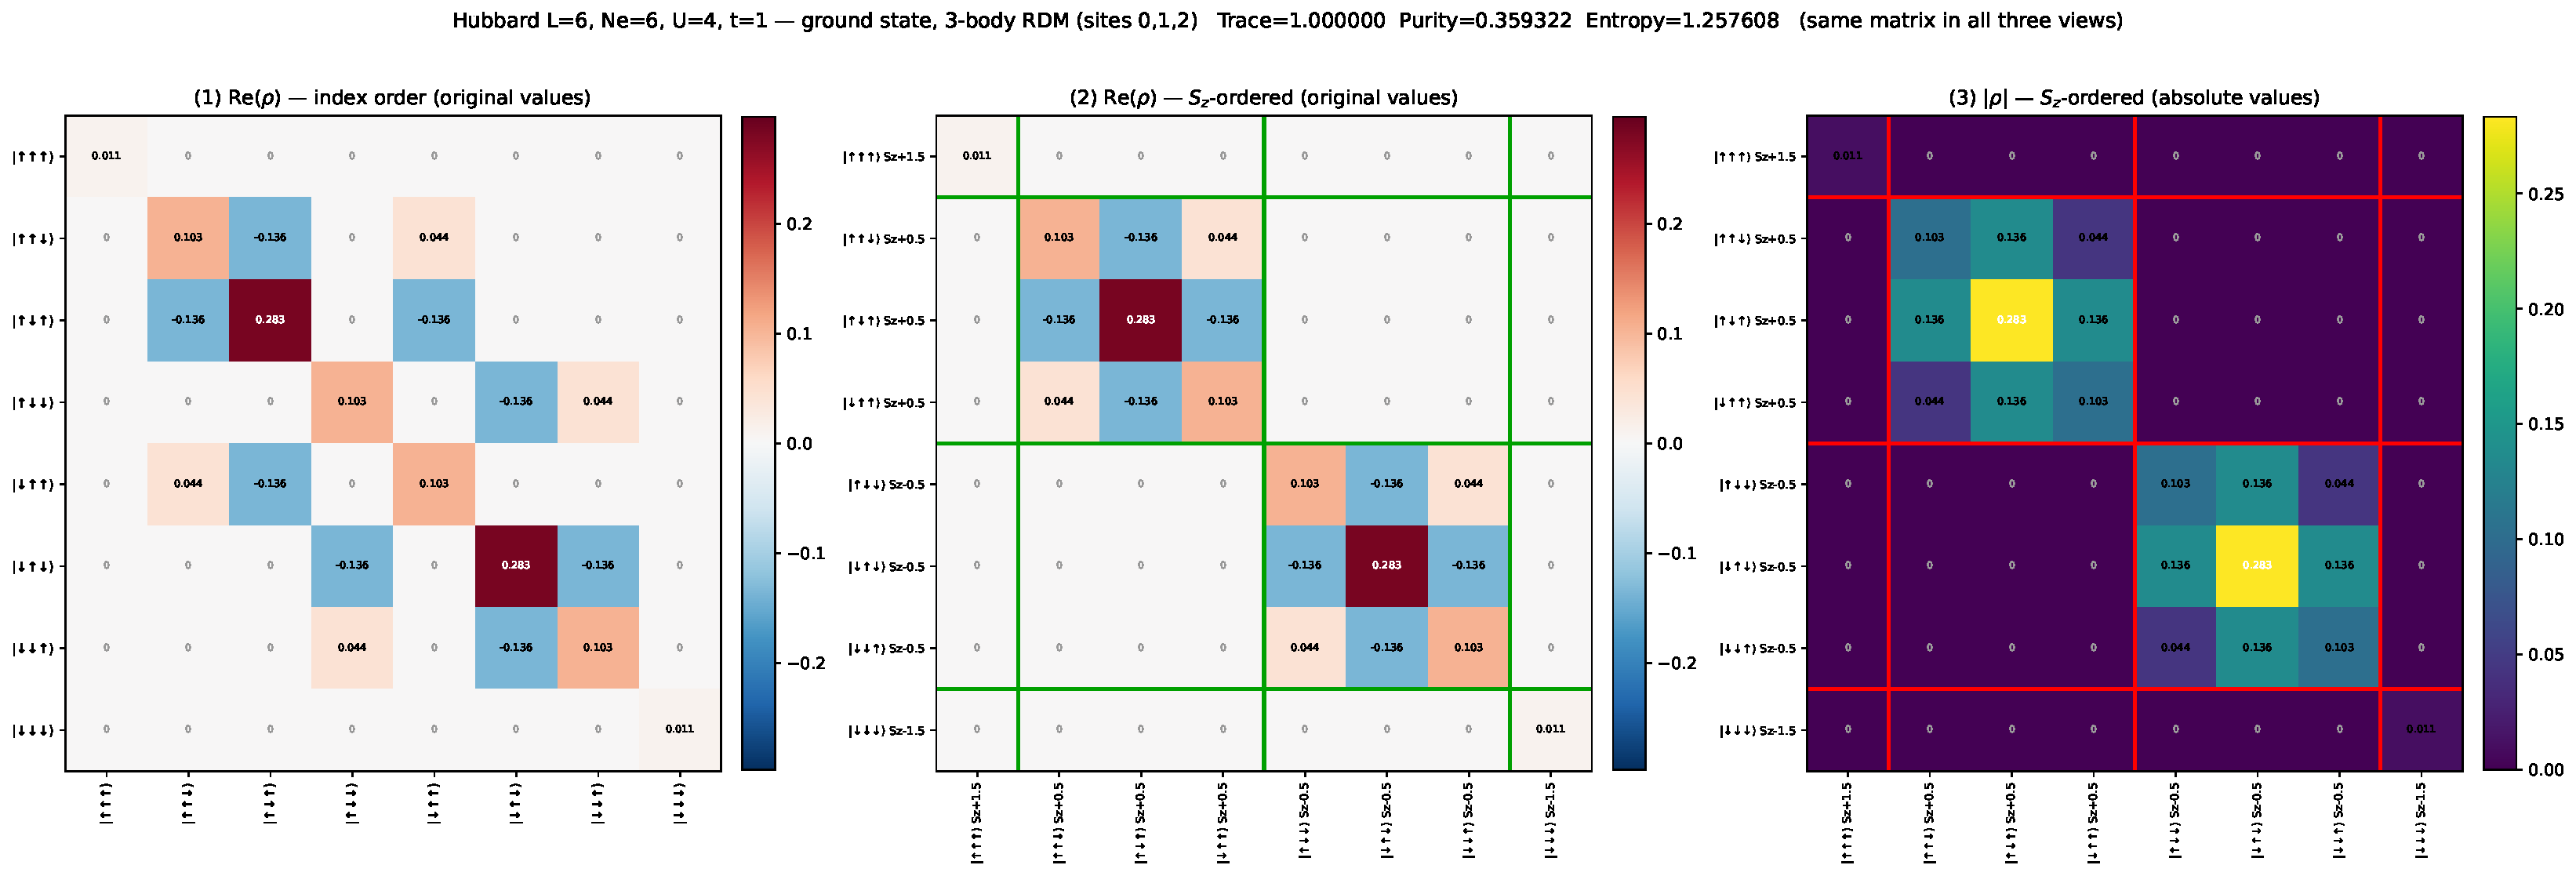
\includegraphics[width=.99\linewidth]{figs/fig_szblocks.pdf}
\end{center}
{\small\textit{One matrix, three views (Hubbard $L{=}6$, ground state,
sites 0,1,2): index order, $S_z$-ordered signed values, $S_z$-ordered
magnitudes. All structure lives inside the $S_z$ blocks.}}
\end{block}

\begin{block}{3. Thermal states for free}
Eigenstate RDMs are temperature-independent; only the Gibbs weights change:
\[
  \rdm(T)=\sum_m p_m(T)\,\rdm[\psi_m],\qquad
  p_m(T)\propto e^{-(E_m-E_0)/T}.
\]
One diagonalisation therefore yields the \emph{entire} temperature sweep —
the controlled path from a pure, strongly entangled ground state to the
separable high-$T$ limit.
\end{block}

\end{column}

% ═════════════════════════════ COLUMN 2 ═════════════════════════════════════
\begin{column}{.32\linewidth}

\begin{block}{4. Hubbard ring: GME across $(t/U,\,T)$}
Half-filled 1-D Hubbard ring ($L$ sites, PBC; $S_z{=}0$ sector and full
Hamiltonian), all $\binom{L}{n}$ clusters per body order $n$:
\begin{center}
  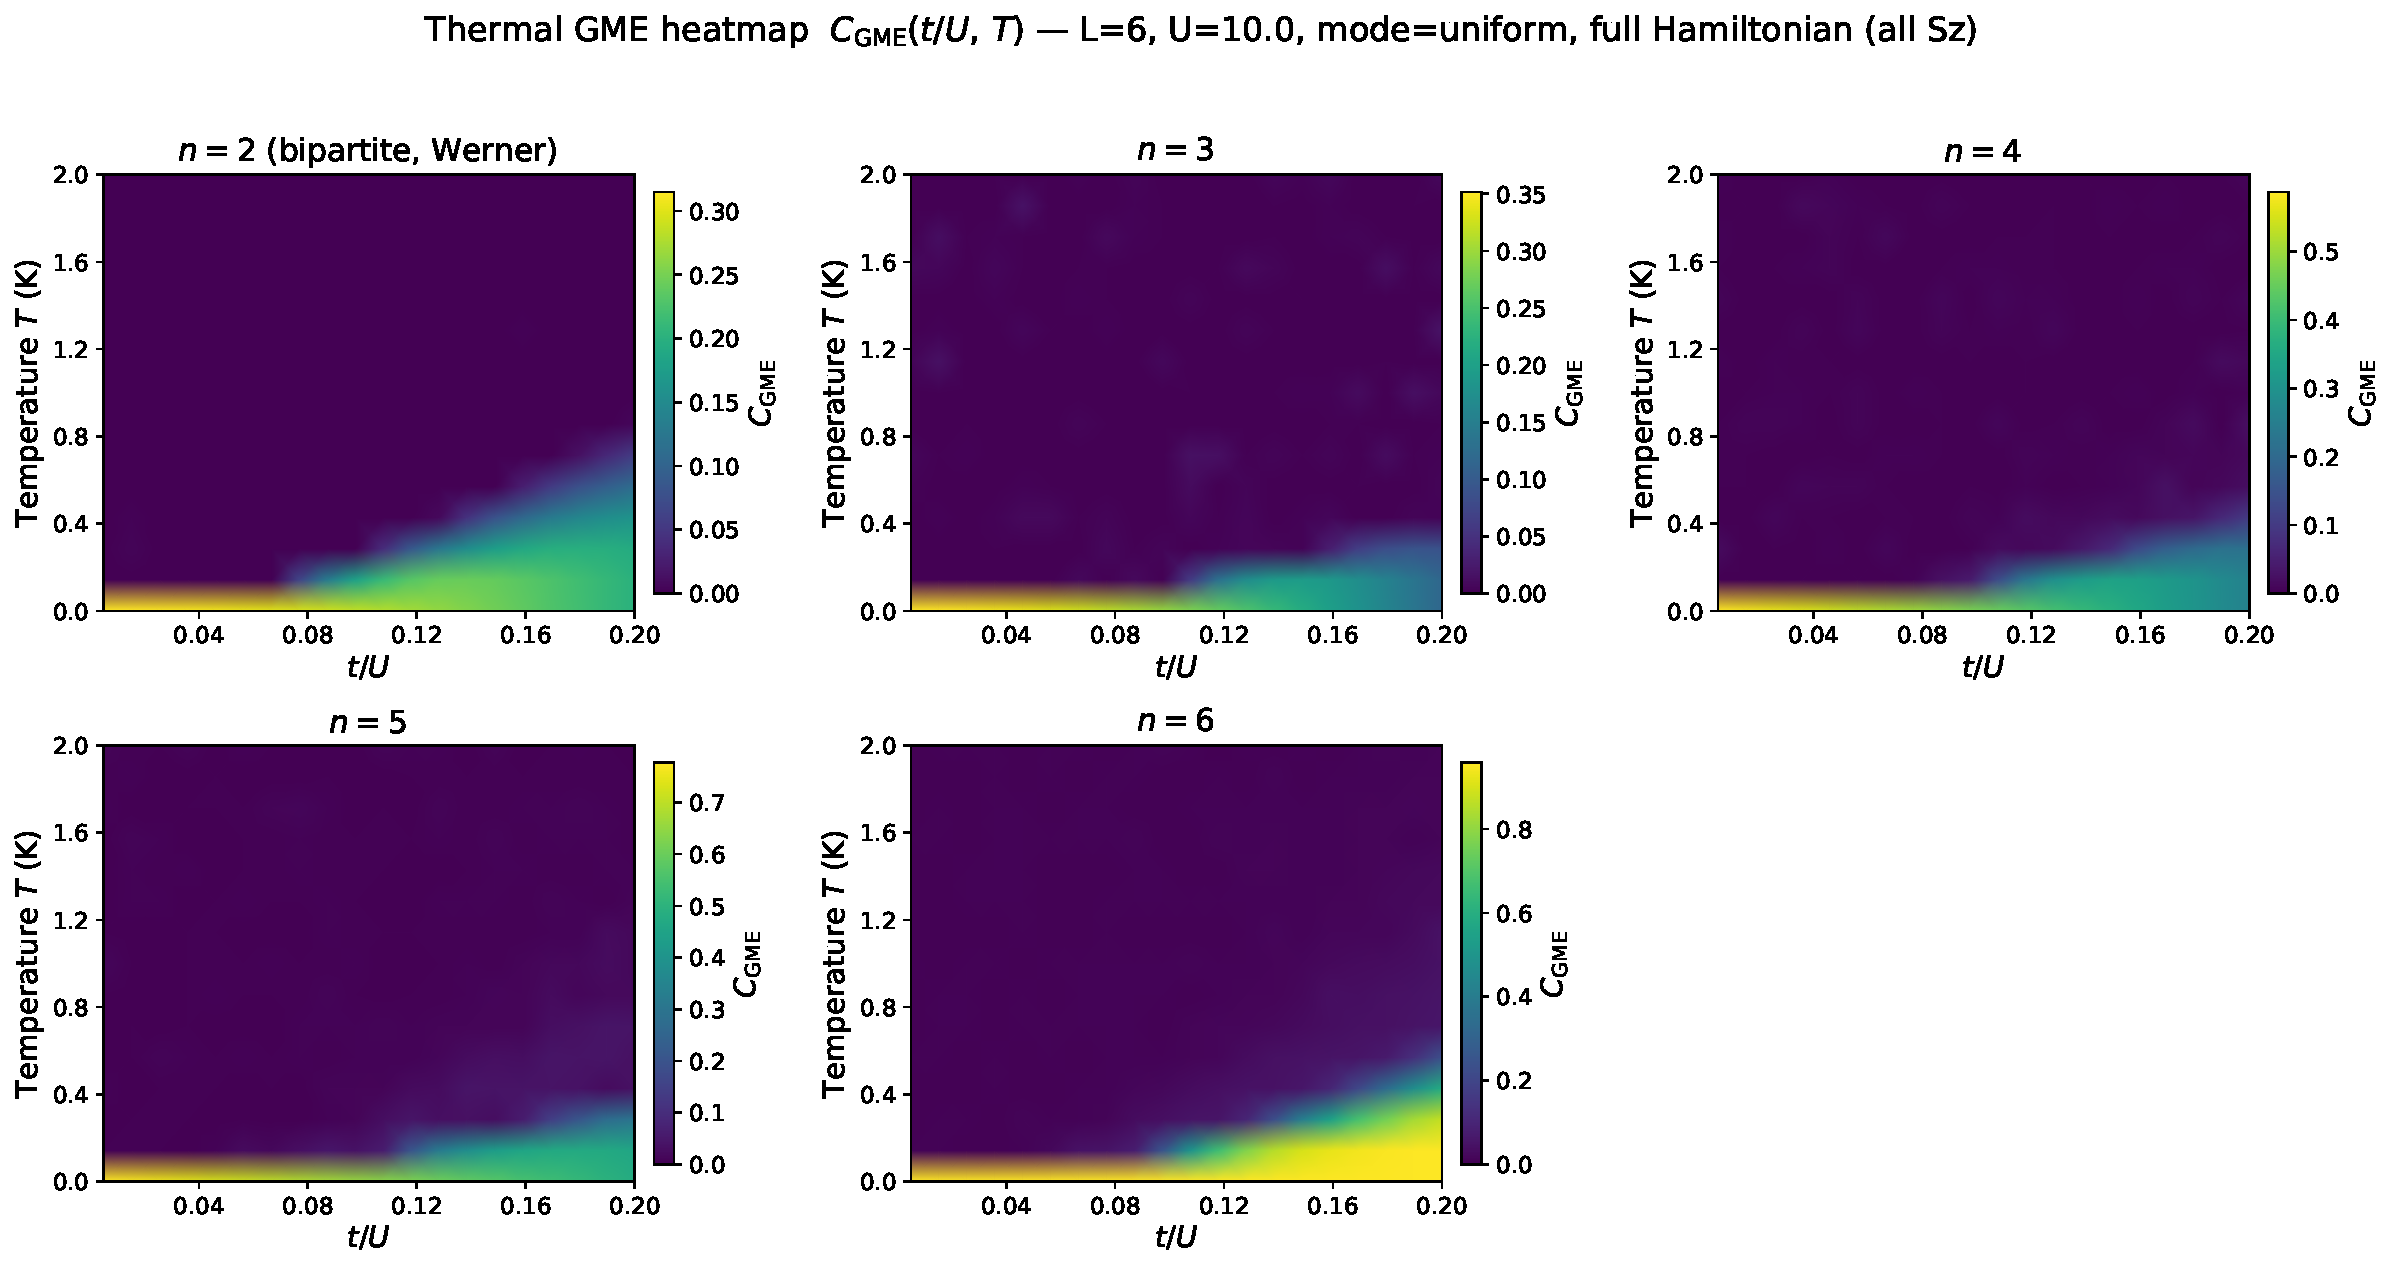
\includegraphics[width=.99\linewidth]{figs/fig_hubbard_heatmap.pdf}
\end{center}
{\small\textit{$\CGME(t/U,\,T)$ per body order $n$ ($L=6$, full
Hamiltonian). Bright bottom band = entangled ground state; dark top =
thermal death.}}
\begin{center}
  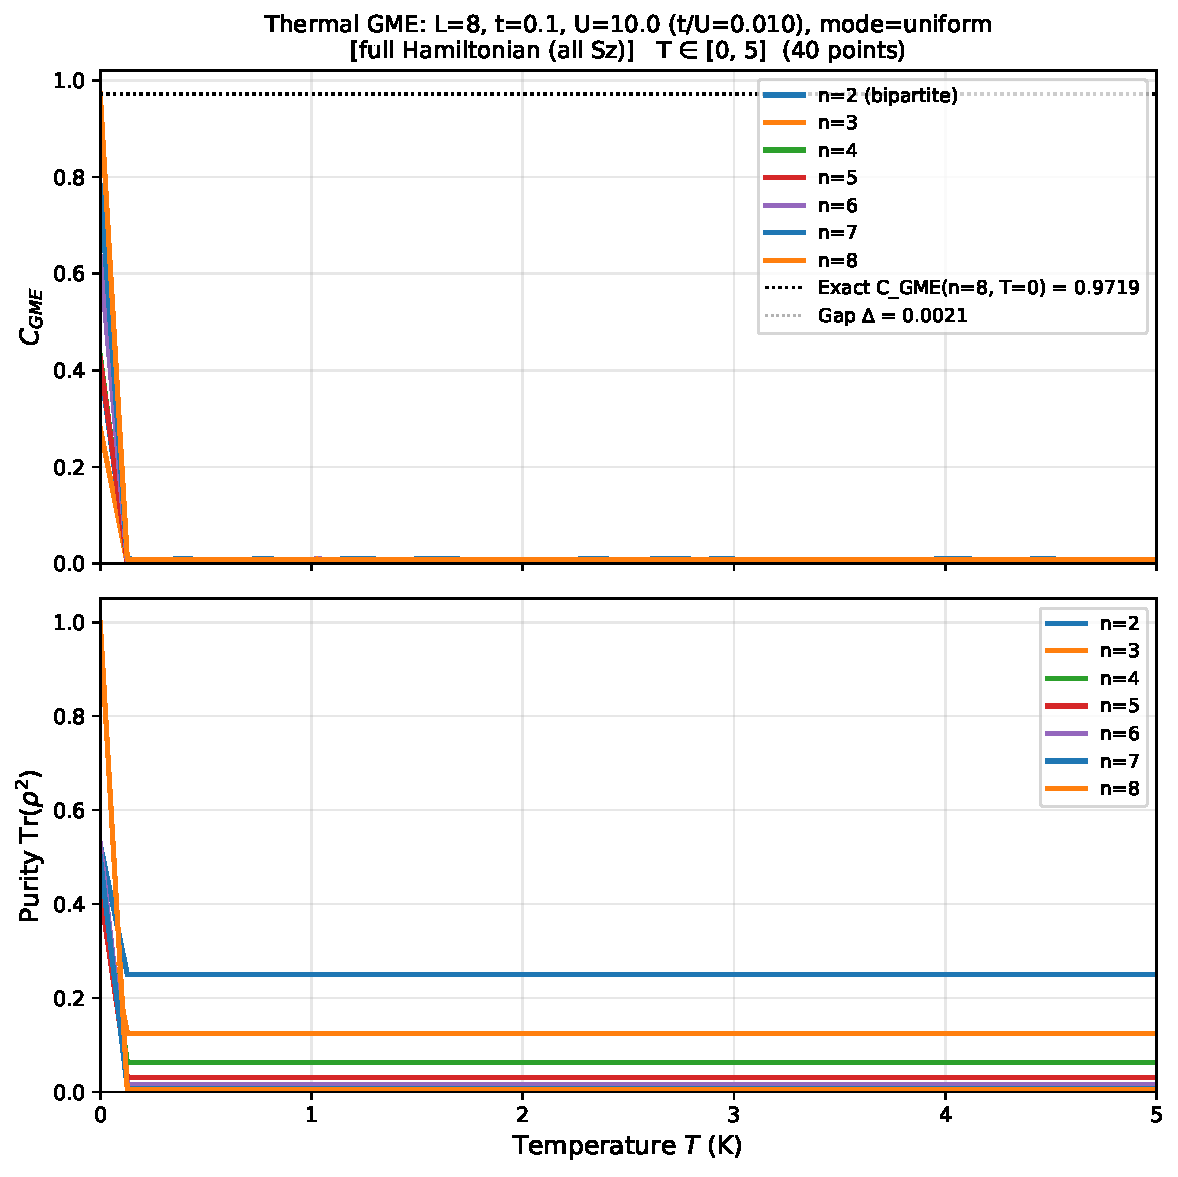
\includegraphics[width=.90\linewidth]{figs/fig_l8_thermal.pdf}
\end{center}
{\small\textit{$L=8$: thermal decay of \CGME{} per $n$ (per-$n$ HPC array
jobs + merged surfaces).}}
\end{block}

\begin{alertblock}{Key findings — Hubbard}
\begin{itemize}
  \item \textbf{Growth with cluster size at $T{=}0$}: whole-ring
        $\CGME\!\approx\!0.96$ ($n{=}L{=}6$), pure-state limit.
  \item \textbf{Thermal death} of GME, with survival temperature set by the
        gap (larger $t/U$ $\Rightarrow$ entanglement survives hotter).
  \item $n{=}2$ reduces exactly to the Wootters concurrence (Werner-state
        form) — an analytic anchor for every pipeline stage.
  \item Near-separable states can show weak \textbf{thermal enhancement} —
        heating \emph{creates} GME when the ground state is almost a product.
\end{itemize}
\end{alertblock}

\begin{block}{5. Scaling strategy}
RDM ``banks'' (per-eigenstate RDMs, cached once per Hamiltonian) make every
analysis reusable; $L=8$ runs as one-job-per-$n$ SLURM arrays
($n=7,8$: $128/256$-dimensional convex roofs). Memory of the full bank scales
as $16^{L}/L$ — $L{=}8$ needs a large-RAM node, $L{=}10$ demands
tensor-network RDMs instead of exact diagonalisation.
\end{block}

\end{column}

% ═════════════════════════════ COLUMN 3 ═════════════════════════════════════
\begin{column}{.32\linewidth}

\begin{block}{6. Benzene: the $\pi$ system as a six-site ring}
CAS$(6,6)$ $\pi$ active space of benzene (cc-pVDZ; exact CASCI ground state,
$E_0=-230.7536$~Ha, gap $0.175$~Ha) — the molecular twin of the $L=6$
Hubbard ring. GME computed in \textbf{two orbital bases} (same energy,
different partition):
\begin{center}
\small
\begin{tabular}{@{}c ccc ccc@{}}
\toprule
 & \multicolumn{3}{c}{\textbf{Canonical MOs}} &
   \multicolumn{3}{c}{\textbf{Pipek--Mezey localized}} \\
$n$ & $\max\CGME$ & mean & \#GME & $\max\CGME$ & mean & \#GME \\
\midrule
3 & 0.074 & 0.009 & 2 & 0.006 & 0.002 & 0 \\
4 & 0.108 & 0.018 & 1 & 0.221 & 0.058 & 3 \\
5 & 0.000 & 0.000 & 0 & \textbf{0.128} & \textbf{0.123} & \textbf{6/6} \\
\bottomrule
\end{tabular}
\end{center}
{\small Double occupancy $\langle D\rangle$: canonical $2.96$ (near-RHF) vs
localized $1.33$ (Hubbard-like). In the \textbf{site-local basis} benzene
reproduces the Hubbard ring's GME pattern — growth with cluster size,
symmetry-uniform values.}
\begin{center}
  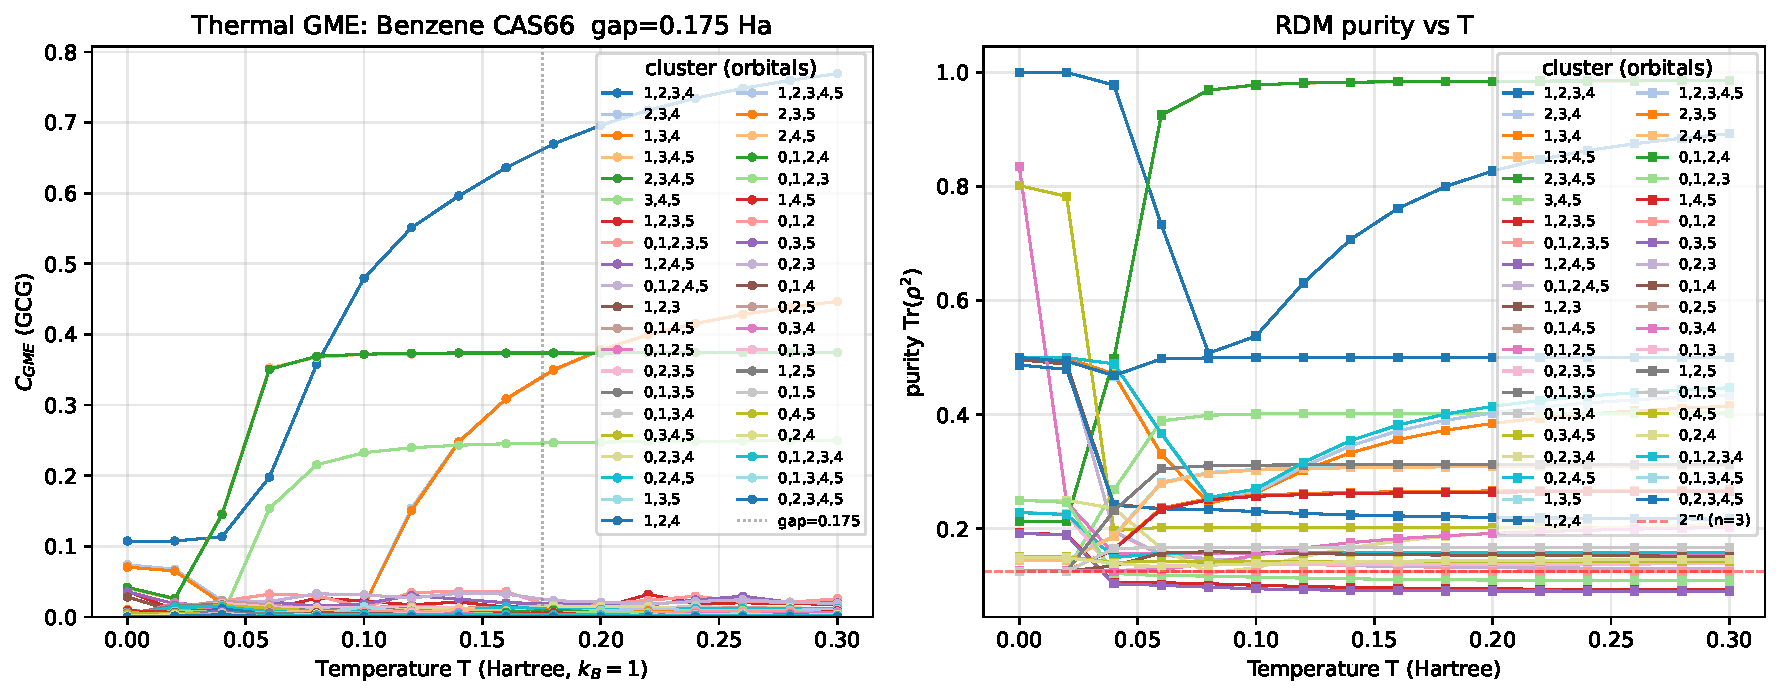
\includegraphics[width=.94\linewidth]{figs/fig_benzene_thermal.pdf}
\end{center}
{\small\textit{Thermal GME of benzene CAS$(6,6)$: Gibbs mixing over CAS
eigenstates. In the canonical basis heating \emph{creates} multi-orbital
GME (near-determinant ground state); localized-basis thermal runs mirror the
lattice behaviour.}}
\end{block}

\begin{block}{7. ML estimation of \CGME{} (surrogate for the convex roof)}
4{,}339 GCG-labelled RDMs ($L{=}2\ldots8$, ground/excited/thermal, both
sectors) train gradient-boosted models on \textbf{$S_z$-block features}
computed from $\rho$ alone (block populations, coherence strengths $\pm$,
block purities — no Hamiltonian parameters, no temperature):
\begin{center}
\small
\begin{tabular}{@{}lccc@{}}
\toprule
 & MAE & $R^2$ & hard-band acc. \\
\midrule
physics baseline (analytic LB) & 0.166 & 0.44 & --- \\
spectral features              & 0.044 & 0.93 & 0.86 \\
\textbf{$S_z$-block features}  & \textbf{0.009} & \textbf{0.997} & 0.93 \\
\bottomrule
\end{tabular}
\end{center}
{\small Coherence-aware, symmetry-informed features are decisive —
spectral (unitary-invariant) features are blind to the off-diagonals where
entanglement lives. Extrapolation to unseen $L$: $R^2\approx0.86$.}
\end{block}

\begin{alertblock}{Conclusions \& outlook}
\begin{itemize}
  \item Exact GME maps for the Hubbard ring across $(n,\,t/U,\,T,\,S_z$
        sector$)$; thermal death/enhancement resolved.
  \item Benzene's $\pi$ system = an effective half-filled six-site ring —
        \emph{visible only in the localized-orbital partition}.
  \item ML surrogate predicts \CGME{} from cheap RDM features
        ($R^2\!\approx\!0.997$), enabling fast pre-screening of sweeps.
  \item \textbf{Next}: decomposition-predicting networks (amortized convex
        roof, certified upper bounds); $n{=}9,10$ via DMRG RDMs;
        Hubbard$\to$molecule transfer tests.
\end{itemize}
\end{alertblock}

\begin{block}{References}
\small
[1] Jungnitsch, Moroder, G\"uhne, PRL \textbf{106}, 190502 (2011).\;
[2] Gray, Banchi, Bayat, Bose, PRL \textbf{121}, 150503 (2018).\;
[3] Chen, Lin, Wei, arXiv:2210.13837.\;
[4] Laskowski et al., PRA (2011), arXiv:1110.4108.\;
[5] [YOUR GCG / GME-measure REFERENCES].
\end{block}

\end{column}
\end{columns}
\end{frame}
\end{document}
